\documentclass[12pt,a4paper,table]{article}

\usepackage[a4paper,
            tmargin=2cm,
            bmargin=2cm,
            lmargin=2cm,
            rmargin=2cm,
            bindingoffset=0cm]{geometry}

\usepackage{lmodern}
\usepackage[T1]{polski}
\usepackage[utf8]{inputenc}
\usepackage{tocloft}
\usepackage{hyperref}
\usepackage{amsmath}
\usepackage{listings}
\usepackage{graphicx}
\usepackage{subfig}
\usepackage{float}
\usepackage{booktabs}

\hypersetup{
    colorlinks,
    citecolor=black,
    filecolor=black,
    linkcolor=black,
    urlcolor=black
}

\newtheorem{definition}{Def}


\begin{document}
    \title {
        Algorytmy Macierzowe \\
        Sprawozdanie 1 \\
        Rekurencyjne mnożenie macierzy

    }

    \author{
        Szymon Paszkiewicz \\
        Przemysław Węglik
    }

    \date{\today}

    \maketitle

    \tableofcontents
    \newpage

    \section{Algorytm Binét'a}

    \subsection{Opis algorytmu}
    Polega na rekurencyjnym rozbijaniu macierzy na 4 mniejsze i 
    obliczaniu wyników dla tych podproblemów. Tam ponownie
    będziemy musieli użyć mnożenia i wykorzystamy procedurę.
    To klasyczne podejście nosi nazwę "divide and conquer".
    Stosujemy wzór:
    $$
    \begin{bmatrix}
        A_{11} & A_{12} \\
        A_{21} & A_{22} \\ 
    \end{bmatrix}
    \times
    \begin{bmatrix}
        B_{11} & B_{12} \\
        B_{21} & B_{22} \\ 

    \end{bmatrix}
    =
    \begin{bmatrix}
        (A_{11}B_{11} + A_{12}B_{21}) & (A_{11}B_{21} + A_{12}B_{22}) \\
        (A_{21}B_{11} + A_{22}B_{21}) & (A_{21}B_{12} + A_{22}B_{22}) \\ 
    \end{bmatrix}
    $$
    
    \subsection{Kod algorytmu}
    \begin{lstlisting}[language=Python]
    def binet_core_algorithm(
                                A: np.ndarray, 
                                B: np.ndarray, 
                                counter: Counter
                            ) -> np.ndarray:
        add = counter.add
        sub = counter.sub
        mul = counter.mul
        if A.size > 1:
            split_at = A.shape[0]//2
            A11, A12, A21, A22 = split(A, split_at, split_at)
            B11, B12, B21, B22 = split(B, split_at, split_at)
            
            C11 = add(binet_core_algorithm(A11, B11, counter), 
                binet_core_algorithm(A12, B21, counter))
            C12 = add(binet_core_algorithm(A11, B12, counter), 
                binet_core_algorithm(A12, B22, counter))
            C21 = add(binet_core_algorithm(A21, B11, counter), 
                binet_core_algorithm(A22, B21, counter))
            C22 = add(binet_core_algorithm(A21, B12, counter), 
                binet_core_algorithm(A22, B22, counter))
            
            return np.concatenate(
                [
                    np.concatenate([C11, C12], axis = 1),
                    np.concatenate([C21, C22], axis = 1)
                ],
                axis = 0)
        else:
            return mul(A, B)
    \end{lstlisting}

    \subsection{Benchmarki}

    \begin{figure}[H]
        \centering
        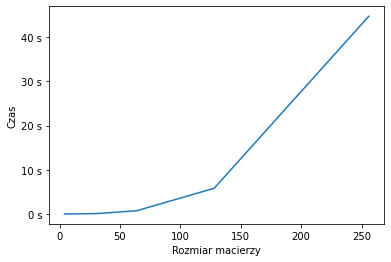
\includegraphics[width=0.6\linewidth]{img/binet_times.png}
        \caption{Wykres czasu od rozmiaru macierzy}
        \label{fig:binet_times}
    \end{figure}

    \begin{figure}[H]
        \centering
        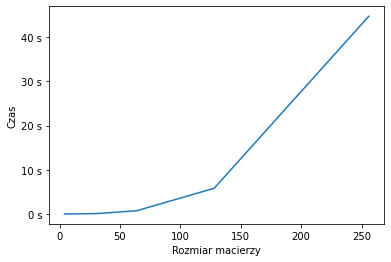
\includegraphics[width=0.6\linewidth]{img/binet_times.png}
        \caption{Wykres ilości operacji od rozmiaru macierzy}
        \label{fig:binet_flops}
    \end{figure}

    \subsection{Analiza złożoności}


    \subsection{Porównanie z matlabem}
    Matlab:
    \begin{lstlisting}[language=Matlab]
    A = [1 3 5; 2 4 6; 3 5 7];
    B = [1 2 3; 4 5 6; 7 8 9];

    disp(A * B);

    % output
    >> matrix_mul
    48    57    66
    60    72    84
    72    87   102
    \end{lstlisting}
    Python:
    \begin{lstlisting}[language=Python]
    A = np.array([[1, 3, 5], [2, 4, 6], [3, 5, 7]])
    B = np.array([[1, 2, 3], [4, 5, 6], [7, 8, 9]])

    print(binet_algorithm(A, B, Counter()))

    # output
    [[ 48  57  66]
    [ 60  72  84]
    [ 72  87 102]]
    \end{lstlisting}
        

\end{document}